\documentclass[12pt,a4paper]{article}
\synctex=1
\usepackage[utf8]{inputenc}
\usepackage[margin=1cm,bottom=2cm]{geometry}
\usepackage{graphicx}
%\usepackage{verbatim}
\usepackage{listings}
\usepackage{multicol}
\usepackage{libertine}
\usepackage{pgfornament}
\usepackage{eso-pic}
\usepackage{textcomp}
\usepackage{courier}
\usepackage[hangul]{kotex}
\linespread{1.3}

\title{
	\centering
	\pgfornament[width=12cm,color=teal]{84}\\
	\vspace{1cm}
	\fontsize{50}{50} \selectfont {시스템 S/W 실습10}\\
	\pgfornament[width=12cm,color=teal]{88}\\
	\vfill}
\author{
	\LARGE
	\begin{tabular}{rl}
		\hline
		학번 : & 2016110056\\ 
		학과 : & 불교학부 \\
		이름 : & 박승원\\
		날짜 : & \today\\
		\hline
	\end{tabular}\vspace{2cm}
	\\
	\includegraphics[width=0.5\textwidth]{/home/zezeon/Dropbox/Photos/logo.jpg}
}
\date{}


\begin{document}
\maketitle
\newpage
\noindent
\lstset{columns=flexible, tabsize=4, frame=single, showstringspaces=false, breaklines=true, upquote=true}

\pagenumbering{gobble}
\lstset{language=C++}
%\begin{multicols}{2}
\begin{enumerate}
\item 다음에 주어진 리눅스 명령을 입력하고, 실습하시오.
\begin{enumerate}
	

\item 별명 (Aliases)
\$alias ls='ls -aF'\\
\$ls *.*

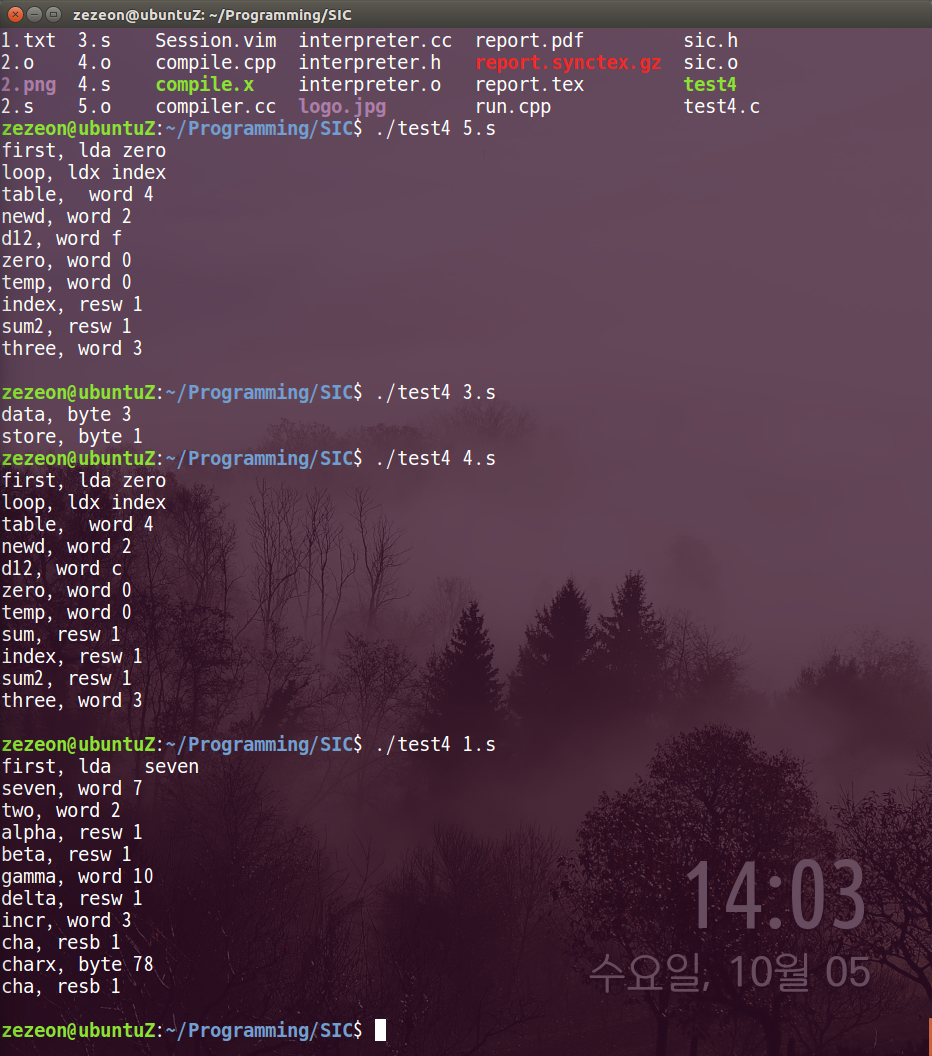
\includegraphics[width=\textwidth]{1.png}

\item 산술계산 : expr
\$x = 1
\$ x=`expr \$x + 1`

2

\item 제어구조
\begin{enumerate}
	\item case .. in .. esac

\lstinputlisting[caption=menu.sh]{menu.sh}
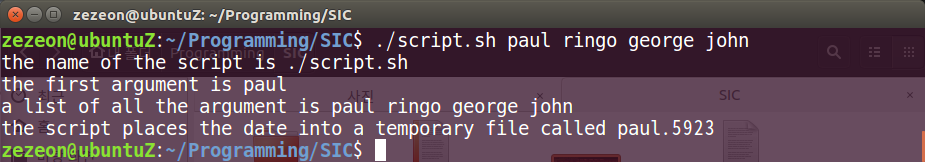
\includegraphics[width=0.5\textwidth]{2.png}

\item for .. do .. done
\lstinputlisting[caption=for.sh]{for.sh}
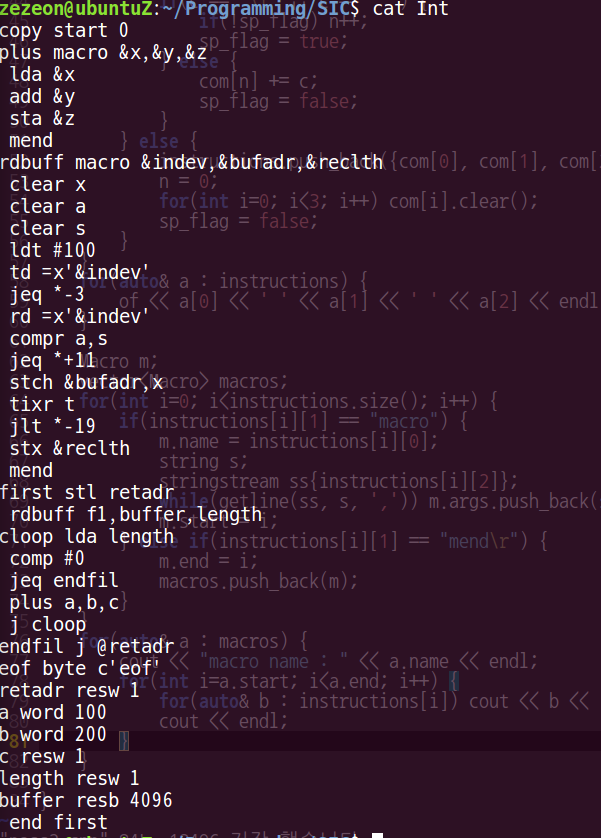
\includegraphics[width=0.5\textwidth]{3.png}

\item if .. then .. fi
\lstinputlisting[caption=fi.sh]{fi.sh}
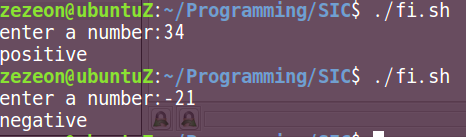
\includegraphics[width=0.5\textwidth]{4.png}
\end{enumerate}
\end{enumerate}
\item 다음에 주어진 Linux 시스템 호출(error 처리)과 관련된 프로그램을 입력하고, 실습하시오.
\lstinputlisting[caption=open.c]{open.c}
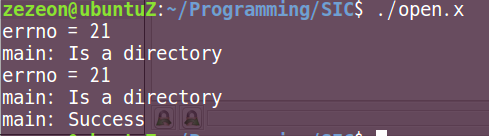
\includegraphics[width=0.5\textwidth]{5.png}
\end{enumerate}
{\Huge소감}
\indent
스크립트가 매우 유용하다는 것을 느꼈다.

\end{document}
